\documentclass[conference]{IEEEtran}
\usepackage{amsmath,amssymb}
\usepackage{booktabs}
\usepackage{graphicx}
\usepackage{url}
\usepackage[hidelinks]{hyperref}
\usepackage{xcolor}
% Mark text still to be written; none may remain at submission.
\newcommand{\todo}[1]{\textcolor{red}{[#1]}}

\title{Additive Block Descent with Evidence-Driven Slots:\\
Twenty Calls to Tune Three Building Energy Controllers}

\author{\IEEEauthorblockN{Zimu Zhang, Runze Liu, Ziqi Ai, Xinlan Hu, Yunyang Wu}
\IEEEauthorblockA{SDM374 Machine Learning System Design, Southern University of Science and Technology}}

\begin{document}
\maketitle

\begin{abstract}
We tune the 21 objective weights of three building energy controllers to minimise the ramping $R$ of the
district's net load, measured by a deterministic black-box simulator. Offline, surrogate models trained on 2,048
rows and searched far from the data were optimistic by 8--43~kWh at the two points we could check, so our best
offline submission was a short, surrogate-vetted step from the best training row ($R=115.68$, below the course
bar of 115.76). Online, with at most 20 sequential calls of 50 points and only the training rows before the first
call, we replace a global surrogate search by an additive block descent: each candidate changes one building, the
next call combines the buildings' improvements, and batch slots are reallocated to the moves that actually lowered
$R$. On the real simulator, all 16 rehearsal runs of the policy family beat our offline result in the first call; the
submitted hybrid policy reaches $R=102.81$ in 1,000 points with the submitted seed, 11.1\,\% below our offline result,
and 105.50 on average over three seeds. The graded package is
deterministic, crash-safe and reproduces every recorded batch bit for bit.
\end{abstract}

\section{Introduction}
\label{sec:intro}
Three buildings on a shared microgrid each run an energy controller that trades off seven objectives (cost,
carbon, peak, discomfort, degradation, ramping and resilience). We tune the $3\times7$ objective weights to
minimise the ramping of the district's net load, which a deterministic black-box simulator measures. Two phases
are graded: an \emph{offline} phase with 2,048 measured rows and two submissions, and an \emph{online} phase in which a
frozen program may call the simulator at most 20 times, sequentially, with up to 50 points per call, using only the
training rows before its first call.

Three properties make the online phase hard for standard Bayesian optimisation~\cite{rasmussen,turbo}. The search
space has 21 weights on three 6-simplices (18 degrees of freedom), the budget is 1,000 points, and the surrogate that would rank
candidates is unreliable exactly where improvements lie: at the two points we could measure offline, surrogate
predictions were 8--43~kWh too optimistic (Section~\ref{sec:problem}). On the other hand, every call returns 50 exact
measurements and is scored by its minimum, so a batch can be designed as a set of experiments rather than a list of
predicted optima. Our contribution exploits this:
\begin{itemize}
\item \textbf{Additive block descent} (Section~\ref{sec:block}). Each candidate except a few combination points
changes the weights of one building only, so its effect is measured in isolation; the next call combines the buildings' improvements, whose value the
additive model predicts from measured effects alone, without a fitted model.
\item \textbf{A controlled evaluation} (Section~\ref{sec:exp}). Complete 20-call rehearsals on the released simulator,
six seeds for v2, v4 and the ablation and three for v1 and the submitted policy, exact permutation tests, and an
ablation that removes the block structure and the two rules that depend on it. We also
report a negative result: evidence-driven slot allocation (Section~\ref{sec:alloc}), which reassigns batch slots by
measured hit rates, changes where points are spent but not the final $R$.
\end{itemize}
The policy is deployed as a deterministic package that recomputes every batch exactly from its log; when the BLAS
configuration matches, the graded run reproduces its rehearsal.

\section{Offline Phase: Surrogates Meet Two Real Points}
\label{sec:offline}
\textbf{Protocol.} All models share one interface (\texttt{fit}, \texttt{predict} with a mean and a standard
deviation) and one evaluation protocol, \emph{frozen-v3.2}: ten fixed train/test splits of the 2,048 rows scored on
local and global ranking, error and the regret of the top-ranked test row (0--100, higher is better). The course
quadratic ridge scores 66.45 (top-1 regret 4.51), ExtraTrees 68.00 (5.85), HistGradientBoosting 72.35 and XGBoost 73.47
(1.07); the gaps are inside the split-to-split standard deviation of about 9. A semi-synthetic study, in which a fitted
model plays the true function, showed that \emph{where} an optimiser lands is set by the surrogate's shape: two
optimisers on the same ridge model reached the same region (regret within 0.25), while switching the surrogate moved the
regret by 5--25.

\textbf{Two real points.} Only the simulator can tell how $R$ behaves outside the data, and the offline phase gave two
such measurements before our second submission (Table~\ref{tab:offline}). The course baseline's $W^\ast$ is a corner of
the simplex where the quadratic surrogate predicted 75.9; it measured 119.09. Our first submission was the consensus
optimum of three tree-based models, which predicted 107--111 and agreed with each other because they had been searched
on their shared error; it measured 119.71. Only ExtraTrees, the model that predicts flat values away from the data, had
the right sign at both points.

\begin{table}[t]
\centering
\caption{Surrogate predictions at the two points measured before our second offline submission (kWh). Best training
row: 115.76.}
\label{tab:offline}
\begin{tabular}{lrr}
\toprule
Model & baseline $W^\ast$ & submission 1\\
\midrule
quadratic ridge (course) & 75.90 & 95.13\\
HistGradientBoosting & 117.62 & 107.80\\
XGBoost & 114.21 & 107.28\\
stacked ensemble & 118.73 & 111.42\\
ExtraTrees & -- & 126.09\\
\midrule
\textbf{measured} & \textbf{119.09} & \textbf{119.71}\\
\bottomrule
\end{tabular}
\end{table}

\textbf{A short, vetted step.} We therefore submitted a step of length 0.05 from \texttt{p01969}, the best and an
isolated training row (nearest neighbour 0.30 away). Among 19,483 random directions that point away from both failed
submissions, we kept the one an ARD Gaussian process~\cite{rasmussen} over additive per-building kernels rated most
confidently (predicted gain $-2.85$, $z=1.90$). The step measured $R=115.68$: below the bar, but the real gain ($-0.08$)
was 35 times smaller than predicted. Offline, the surrogates could at best tell the direction of a short step, never its
size.

\section{What the Simulator Looks Like}
\label{sec:landscape}
The simulator was released after the offline phase, and the TA confirmed that local runs may be used to choose models,
policies and their constants, provided the submitted code uses only the training rows before its first call and embeds
no locally measured point, value or weight. We used this in two studies. Both inform the design of
Section~\ref{sec:strategy}; neither feeds data into it.

\textbf{The surrogate cannot see the low region.} On held-out training rows our additive ARD kernel beats generic
21-dimensional ARD kernels (MAE 3.40 against 4.74--5.98), and its 95\,\% intervals cover 94.8\,\% of held-out rows. Its
constant prior mean, however, fails away from the data: the 200 lowest of 6,548 locally measured points ($R\approx105.1$,
about 1.9 training spacings out, on the simplex boundary) are predicted at $124.4\pm8.8$. Trend terms, a log target and
per-building length scales did not change this. Reaching the low region is an exploration problem, not a modelling one.

\textbf{Structure of $R$.} An unrestricted local search (about 22,500 simulator evaluations, exploration only) found
$R=102.10$ and four regularities: (i) $R$ is additive over buildings within a basin (error about 0.03) but couples by up
to 0.85 across basins, and each building has several near-equivalent valleys; (ii) the ramping weight is the sensitive
coordinate and $R$ is terraced, with plateaus 0.02--0.2\,\% of a weight wide; (iii) small weights act as switches:
shares of $10^{-5}$ to $3\times10^{-3}$ on otherwise unused objectives lower $R$ by flipping near-tied hourly decisions,
while shares below $10^{-6}$ equal zero; (iv) the last gains came from systematic one-coordinate scans that random
perturbations missed. Additivity was already visible in the training rows: a building-additive model cross-validates as
well as an unconstrained one ($R^2$ 0.846 vs.\ 0.844).

\section{Online Policy: Additive Block Descent}
\label{sec:strategy}
The policy sees only the 2,048 training rows and the results of its own calls. It keeps a \emph{base} $B$, the best
point measured so far (at call 1, the best training row, which is never resent), and proposes 50 new points per call.

\textbf{Blocks and combinations.} Every candidate changes the 7-weight block of exactly one building and keeps the
other two at the base, so $R(\text{candidate})-R(B)$ measures that block's effect alone. The next call builds a new
base from the best improving block of each building, plus up to six other combinations of improving blocks; under
additivity these are predicted by summing block effects. One batch thus advances three 7-dimensional searches at once,
a block-coordinate descent~\cite{bcd} that uses additivity the way additive Bayesian optimisation does~\cite{addgp},
but on measured rather than modelled block effects.

\textbf{Moves.} The remaining slots are split across buildings among four move classes:
\emph{model} picks, the lowest lower confidence bound (mean $-$ std) among 1,500 perturbations of the block, from a
navigation surrogate that adds an ARD Gaussian process on the 600 rows nearest the base to a ridge trend fitted on all
data (features: the degradation/ramping ratio and log shares, CV $R^2$ 0.844 vs.\ 0.775 for raw weights);
\emph{random} moves at a per-building trust scale that grows by 1.5 after a success and shrinks by 0.6 after a
failure, within $[0.01,1]$, as in trust-region BO~\cite{turbo}; \emph{fine} moves (small multiplicative steps, setting
a minor weight to zero, or setting it to a tiny share drawn from the 0.1--10\,\% quantiles of training weights,
$1.6\times10^{-6}$ to $7.2\times10^{-3}$); and, from call 9, \emph{scans}: one-coordinate steps just outside the known
plateau, plus the previous call's improving coordinates re-applied to the new base. Calls 1--6 bias the shift
target toward objectives whose share correlates negatively with $R$ in the training rows.

\textbf{Evidence-driven slots (v4).} Three rules use the run's own results only. A one-coordinate move that returns
exactly $R(B)$ marks a plateau, and no later move is proposed inside the widest such interval (in earlier versions
30\,\% of late points repeated a value already seen). Slot shares per building follow each class's hit rate over the
last four calls, $(h+1)/(n+5)$, with floors of 0.25 for model picks and 0.10 for the others (model picks hit 9\,\% of the
time but had held 42\,\% of the slots). Candidates that repeat a training row or a sent point are never proposed, so
every call sends 50 new points.

\textbf{Hybrid replacement (h7, submitted).} Calls 1--11 are v4 unchanged. From call 12 the policy takes v4's full
50-point batch and replaces at most 12 slots of the classes that produced none of v4's late improvements (fine and
zero moves) by multiscale candidates: \emph{coarse} single-coordinate factors in $\{0.45,\dots,3.0\}$ to cross
plateaus, \emph{block} moves of 2--3 coordinates, and \emph{restarts} towards a low training block or this call's elite
block. A building's block step widens from 0.22 to 0.35 after three calls without improvement. Every random draw is
seeded by (seed, call), so the batch sequence is a pure function of the seed and the measured values.

\section{Rehearsals on the Real Simulator}
\label{sec:results}
Each rehearsal is a complete 20-call, 1,000-point run of a policy on a local copy of the released simulator
(sha256-pinned), with the policy's own pre-submit screen and log. Table~\ref{tab:online} lists the best $R$ of every
run; Fig.~\ref{fig:convergence} shows the best value per call.

\begin{table}[t]
\centering
\caption{Best $R$ (kWh) after 20 calls $\times$ 50 points on the real simulator, by policy and seed. Best offline
result: 115.68; best training row: 115.76.}
\label{tab:online}
\setlength{\tabcolsep}{4pt}
\begin{tabular}{lrrrr}
\toprule
Policy & seed 2026 & seed 7 & seed 11 & mean\\
\midrule
v1: block descent & 107.03 & 107.21 & 106.43 & 106.89\\
v2: v1 + training shift bias & 106.95 & 105.11 & 107.49 & 106.52\\
v4: v2 + evidence-driven slots & 108.05 & 103.28 & 105.44 & 105.59\\
v5: v4 + vertex probes, lanes & 106.17 & 106.18 & 106.44 & 106.26\\
v6: v4 + lanes when stalled & 107.41 & 106.48 & 106.68 & 106.86\\
v4, fixed-constant GP & 106.43 & 105.08 & 107.15 & 106.22\\
\textbf{h7: v4 + hybrid (submitted)} & 107.81 & \textbf{102.81} & 105.87 & 105.50\\
\bottomrule
\end{tabular}
\end{table}

\begin{figure}[t]
\centering
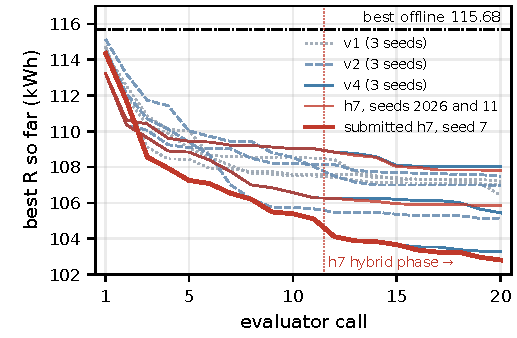
\includegraphics[width=\columnwidth]{figures/convergence.pdf}
\caption{Best measured $R$ per call. Thin lines: v1, v2 and v4, three seeds each; red: the submitted h7 (thick: seed 7,
the submitted seed; thin: seeds 2026 and 11), identical to v4 with the same seed up to call 11. Source: logs in
\texttt{analysis/online\_rehearsal/}, \texttt{analysis/online\_v7/} and \texttt{analysis/online\_v7\_seeds/} (real
simulator, no surrogate values).}
\label{fig:convergence}
\end{figure}

\textbf{Every run beats the offline result in the first call.} All 16 runs of v1--v6 send a first batch whose minimum
lies between 113.2 and 115.1, below our offline 115.68, using only the training rows. Most of the descent happens in
calls 1--5 (to 107--110), after which gains shrink to tenths of a kWh per call.

\textbf{Seeds matter as much as variants.} Variant means lie within 105.6--106.9 while the seeds of one variant span
up to 4.8~kWh (v4: 103.28--108.05), so with three seeds no variant is established as better than v4. Two attempts to
avoid early commitment to one ``form'' per building (v5, v6) and a surrogate with fixed hyperparameters did not help.
The move statistics explain why v4 kept its place: over three seeds, the share of points that beat their call's base was
3.0\,\% for model picks, 7.6\,\% for random moves, 8.8\,\% for fine moves and 7.7\,\% for scans, and scans produced most late
gains. Combinations confirmed additivity online: measured minus predicted had median $+0.013$ and MAE 0.22 over 214
points, whereas the surrogate's own picks landed on average 3.6 above their prediction.

\textbf{The submitted policy.} h7 with seed 7 reaches 102.81 (Fig.~\ref{fig:batches}), 0.47 below v4 with the same seed;
the two runs are identical up to call 15 and diverge from call 16, and the single largest new contribution is one coarse
move at call 19 ($-0.28$). Because h7 was designed on that seed's log, we then ran the graded package unchanged on
seeds 2026 and 11. In calls 1--11 it sends the same batches as v4 and every point gets the same $R$ (apart from a
last-bit difference in four weight vectors and one swapped tie), so the comparison is paired. In calls 12--18 h7's best
value is at or below v4's on all three seeds; after call 20 it is 0.24 below v4 on seed 2026 and 0.43 above on seed 11,
where v4's last two calls dropped from 106.02 to 105.44. The paired mean difference is $-0.09$ ($-0.47$, $-0.24$,
$+0.43$), well inside the seed spread: h7 brings late gains forward but is not shown to end lower than v4.

\begin{figure}[t]
\centering
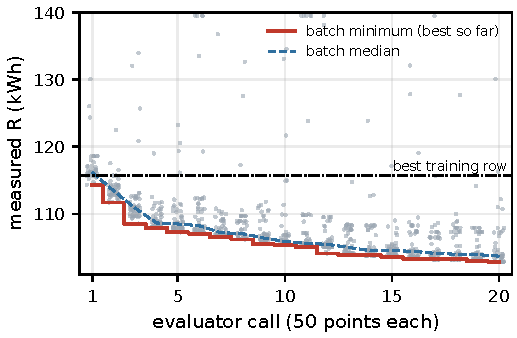
\includegraphics[width=\columnwidth]{figures/h7_batches.pdf}
\caption{All 1,000 measured points of the submitted run (h7, seed 7; values above 139.5 clipped). The score of a call is
its minimum; the batch median stays high because most slots probe, and only the minimum needs to be low.}
\label{fig:batches}
\end{figure}

\section{The Graded Run Is the Rehearsed Run}
\label{sec:runner}
Because the simulator is deterministic, a deterministic policy makes the graded result equal to its rehearsal,
provided the course computer emits the same batches. The graded package is a standalone folder built on the course
\texttt{run.py} loop and launched with one command (\texttt{uv run run.py}); it holds the policy, its constants with
their sources, the 2,048 training rows and a lock file (Python 3.11, NumPy 1.24.4, scikit-learn 1.2.2), and no
pretrained model: the surrogate is refitted from scratch on every call.

\textbf{Determinism.} All randomness derives from (seed, call). Linear-algebra rounding still depends on the BLAS
kernel and thread count, and the GP hyperparameter fit amplifies it to about 0.01 of predicted $R$, enough to swap a
selected candidate. The package therefore fixes the OpenBLAS kernel and thread count before NumPy is imported and stops
if the runtime reports anything else. \texttt{run.py verify} recomputes every batch from a recorded log without the
simulator; for the submitted run all 20 calls match exactly (max $|\Delta W|=0$).

\textbf{Crash safety and budget.} Before each simulator call the batch is written and flushed as \emph{sent}; the
call's checkpoint (weights, raw simulator output, $R$, policy and RNG state, hashes of data, code and simulator) is
written to a temporary folder and renamed only when complete, with a manifest that chains the previous call's hash. A
batch that was sent but returned no $R$ counts as a used call and is never resent, because the simulator charges a call
when it starts. A batch rejected by the simulator's input check (exit code 2) is not charged, but the run still stops
there for a person to decide: in our seed runs, \texttt{solver.exe} launched from a host with an attached console failed
on valid batches with the same exit code and \emph{was} charged. The quota file is never touched, and a simulator
binary whose hash differs from the released one is reported in every checkpoint.

\textbf{Development framework.} Before the package, a shared library gave every surrogate, optimiser and policy one
registry and interface, every experiment a run folder with configuration, commit and dataset hash, and the online loop
an append-only call log, an attempt journal and resumable state; the studies in this report were run on it and on the
rehearsal harness, and each number is traceable to a committed log~\cite{repo}.


\section{Discussion and Conclusion}
\label{sec:discussion}
\textbf{What worked.} The decisive step was not a better surrogate but a search structure that the measurements
supported: additivity over buildings turned one 21-dimensional problem into three 7-dimensional ones advanced in
parallel inside every batch, and per-move hit rates told the policy where its 50 slots paid off. The surrogate
remained useful as one move among several, not as the arbiter of the batch.

\textbf{Limits.} (i) Every policy comparison uses at most three seeds, while one policy's seeds span up to 4.8~kWh;
no variant is established as better than v4. h7 gained 0.47 over v4 on the seed used to design it, but only 0.09 on
average over three paired seeds, and lost on one (Section~\ref{sec:results}). (ii) The seed and the policy were chosen on local runs of the released simulator, which
the TA confirmed as allowed; the submitted code contains no locally measured point, value or weight, but the
expected graded score is the seed spread, not the best seed. (iii) Bit-for-bit reproduction across machines depends on
the BLAS kernel and thread count; the package pins and checks both, but the course computer's result was not
available at the time of writing.

\textbf{Conclusion.} Under a 1,000-point budget the policy family lowers $R$ from the best training row (115.76) to
102.8--108.0 on the real simulator, against 115.68 for our best offline submission and 119.09 for the course
baseline. The lesson that carries over is to spend the budget where measurements, not model predictions, show
progress, and to make the run that is graded the run that was rehearsed.

\bibliographystyle{IEEEtran}
\begin{thebibliography}{9}
\bibitem{rasmussen} C.~E. Rasmussen and C.~K.~I. Williams, \emph{Gaussian Processes for Machine Learning}. MIT Press, 2006.
\bibitem{turbo} D.~Eriksson, M.~Pearce, J.~Gardner, R.~D. Turner, and M.~Poloczek, ``Scalable global optimization via local Bayesian optimization,'' in \emph{NeurIPS}, 2019.
\bibitem{addgp} K.~Kandasamy, J.~Schneider, and B.~P{\'o}czos, ``High dimensional Bayesian optimisation and bandits via additive models,'' in \emph{ICML}, 2015.
\bibitem{bcd} S.~J. Wright, ``Coordinate descent algorithms,'' \emph{Mathematical Programming}, vol.~151, no.~1, pp.~3--34, 2015.
\bibitem{repo} SDM374 Project~1 team repository: decisions log (\texttt{docs/decisions.md}), studies under \texttt{analysis/}, graded package \texttt{submission/}, 2026.
\end{thebibliography}
\end{document}
